% --- CHUNK_METADATA_START ---
% needs_review: True
% src_checksum: 5da0735687c2aea3697e5e896ffcb2de79d53828c4ce70778e3f5615aecdb14a
% --- CHUNK_METADATA_END ---
\chapter{Euclidean Spaces}% --- CHUNK_METADATA_START ---
% needs_review: True
% src_checksum: 09c6effe383b397c2e287b2302b5c82f4782172b70cdf3be336a68a99ec35441
% --- CHUNK_METADATA_END ---
“Classical” linear algebra deals with vector spaces, where we only talk about linear combinations, subspaces, bases, matrices, etc. At some point, this is no longer sufficient. To be able to explore stronger, more complex, and useful notions, we will need to calculate the length of a vector, the angles between two vectors, the relative positioning between vectors, etc. To be able to study these concepts, we introduce the notion of a dot product (bilinear form) and then the vector spaces equipped with this product.

This chapter is devoted to the study of the two main notions:% --- CHUNK_METADATA_START ---
% needs_review: True
% src_checksum: 70055e76d35e68266dcc2b09983fa30f0cc425313d489a398c66762a9624032b
% --- CHUNK_METADATA_END ---
\begin{itemize}
    \item scalar products
    \item Euclidean spaces
\end{itemize}% --- CHUNK_METADATA_START ---
% needs_review: True
% src_checksum: 479ce8267a8dc66449e53b838492edeab11f9f116eed87da087547c1cd388ae6
% --- CHUNK_METADATA_END ---
\section{Introduction}% --- CHUNK_METADATA_START ---
% needs_review: True
% src_checksum: 0ac44e2012e6f37806b8ec7c72ad867302be795f6c99ca78cd8ba87ccba55dd5
% --- CHUNK_METADATA_END ---
The vector spaces considered in this chapter are real. We assume that $E$ is an $\R$-vector space.

Scalar product:% --- CHUNK_METADATA_START ---
% needs_review: True
% src_checksum: aac3ae1bec48ecd43cdb867de27dbe9d4e32a291690935f3e07ad94ea30b3963
% --- CHUNK_METADATA_END ---
\begin{definition}
    A bilinear form on $E$ is a map
    \begin{align*}
        B: E \times E &\longrightarrow \R \\
        (u, v) &\longmapsto B((u, v))
    \end{align*}
    that satisfies the following conditions $\forall u, v, w \in E$ $\forall \lambda \in \R$:
    \begin{enumerate}
        \item $B(u + \lambda v, w) = B(u, w) + \lambda B(v, w)$
        \item  $B(u, v + \lambda w) = B(u, v) + \lambda B(v, w)$
    \end{enumerate}
    B is said to be
    \begin{enumerate}
        \item symmetric if $B(u, v) = B(v, u)$  $\forall u, v \in E$
        \item positive if $B(., u) \ge 0 \, \forall u \in E$
        \item defined if $B(u, u) = 0 \iff u = 0$
    \end{enumerate}
\end{definition}% --- CHUNK_METADATA_START ---
% needs_review: True
% src_checksum: b3e3014d86bf527aed2249534faff461531a00e3c7469faa8feaef31f7788090
% --- CHUNK_METADATA_END ---
\begin{notation}
   Scalar product is denoted: $<u, v>$ 
\end{notation}% --- CHUNK_METADATA_START ---
% needs_review: True
% src_checksum: 8c68c516bc5901f21ff7541f291db7303a684176baa8fee049e9397452534c86
% --- CHUNK_METADATA_END ---
\begin{eg}.
   \begin{enumerate}
       \item $E = \R^n$,  $X = (x_1, \ldots, x_n), Y = (y_1, \ldots, y_n) \in E$\\
           \[
               <X, Y> := \sum_{n=1}^{n} x_iy_i
           \] 
           It is called the "canonical (or usual) scalar product".
        \item $E = \R^2$ and  $<X, Y> = 2x_1y_1 + x_2y_2$
        \item $E = \mathcal{C}^0([-1, 1], \R) \ni f, g$ (a space of continuous functions)
            \[
                <f, g> := \int_{-1}^{1} f(t) \cdot g(t) \: d{t} 
            \] 
        \item $E = \mathcal{M}_n(\R) \ni A, B$
             \[
            <A, B> := Tr(A^tB)
            \] 
   \end{enumerate} 
\end{eg}% --- CHUNK_METADATA_START ---
% needs_review: True
% src_checksum: 3754243cd92b07a4e8a3690f08a016f59688f2b965a017a38bca50239762e19f
% --- CHUNK_METADATA_END ---
\begin{prop}
    A non-zero vector space has an infinite number of different scalar products.
\end{prop}% --- CHUNK_METADATA_START ---
% needs_review: True
% src_checksum: 73752ce65fbe2fdff7cab331cd5cc247e172ed8b55063a0cfebe8d6a4a21be40
% --- CHUNK_METADATA_END ---
\begin{definition}
    A Euclidean space is a pair $(E, < . >)$ where $E$ is a $\R$-vector space \underline{of finite dimension} and $< . >$ is an inner product on $E$.
\end{definition}% --- CHUNK_METADATA_START ---
% needs_review: True
% src_checksum: de6e7256acedf77ba6b59dd8c8638e3b17598fcb2783a559a6ba2e747ecc603d
% --- CHUNK_METADATA_END ---
\begin{property} Let $(E, < . >)$ be a Euclidean space. We define:
    \[
    \|X\| := \sqrt{<X,X>} \qquad X \in E 
    \] 
    the norm (or length) of $X$. (It is well defined because $<., .>$ is always positive)
\end{property}% --- CHUNK_METADATA_START ---
% needs_review: True
% src_checksum: a0c34c74b776c4b2712e0bc68ea2baf5a169429392c9041fa9951ee767e094fd
% --- CHUNK_METADATA_END ---
\begin{property}
   Let $X, Y \in E$ be, then:
   \[
       \|X + Y\|^2 = \|X\|^2 + 2\scalair{X, Y} + \|Y\|^2
   \] 
\end{property}% --- CHUNK_METADATA_START ---
% needs_review: True
% src_checksum: 8432f24eca144a9f41a6cbb5161d6ea135f840aad65be511c92557c145409cf5
% --- CHUNK_METADATA_END ---
\begin{proof}
   \begin{align*}
       \|X + Y\|^2 = \sqrt{\scalair{X + Y, X + Y}}^2 &= \scalair{X + Y, X + Y} \\ 
                                                     &= \scalair{X, X + Y} + \scalair{Y, X + Y}  \\
                                                     &= \scalair{X, X} + \scalair{X, Y} + \scalair{Y, X} + \scalair{Y, Y}\\
                                                     &= \|X\|^2 + 2\scalair{X, Y} + \|Y\|
   \end{align*} 
\end{proof}% --- CHUNK_METADATA_START ---
% needs_review: True
% src_checksum: 01d462ad6bb3b1ce2908c760049b50ee548204ecba31f845da8c1db0f8bf13f6
% --- CHUNK_METADATA_END ---
\begin{lemma}\label{lemma:inegalite-cauchy-schwarz} Cauchy-Schwarz inequality
   We have
   \[
   |<u, v>| \le \|u\| \cdot \|v\| \qquad \forall u, v \in E
   \] 
   with equality if and only if $u$ and  $v$ are collinear, i.e  $\exists \, t \in R$ such that $u = tv$ or  $v = tu$
\end{lemma}% --- CHUNK_METADATA_START ---
% needs_review: True
% src_checksum: dd7937806464a5e6da7e6b458df5a7ae1a082e9a65aec713595521a1e6323273
% --- CHUNK_METADATA_END ---
\begin{explanation}
   If $v = 0$, clear\\
   If $v \neq 0$ we consider $\forall t \in \R$
   \begin{align*}
       \|u + tv\|^2 &= <u + tv, u + tv>\\ 
                    &= <u, u + tv> + t<v, u + tv>\\
                    &= <u, u> + t<u, v> + t<v, u> + t^2<v, v>\\
                    &= \|u\|^2 + 2t<u, v> + t^2 \|v\|^2 = f(t)
   \end{align*}
   \begin{center}
       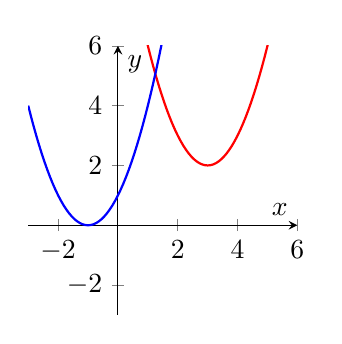
\begin{tikzpicture}
           \begin{axis}[
               axis lines = center,
               xlabel = $x$,
               ylabel = $y$,
               samples = 100,
               domain = -3:6,
               xmin = -3, xmax = 6,
               ymin = -3, ymax = 6,
               width=5cm,
               height=5cm
               ]
               \addplot[red, thick] {(x - 3)^2 + 2};
               \addplot[blue, thick] {(x + 1)^2};
           \end{axis}
       \end{tikzpicture}
   \end{center}
Case 1: $f(t)$ has no distinct roots
\begin{align*}
    &\Delta = 4<u, v>^2 = 4\|u\|^2\|v\|^2 \le 0\\
    \implies & <u, v>^2 \le \|u\|^2 \cdot \|v\|^2\\
    \implies & |<u, v>| \le \|u\|\|v\|
\end{align*}
Case 2: $f(t)$ has only one root:\\
\begin{align*}
    &\Delta = 0\\
    \implies & \exists t \in \R \text{ tq } \|u + tv\|^2 = 0\\
    \implies &u + tv = 0 \implies u = -tv
\end{align*}
\end{explanation}% --- CHUNK_METADATA_START ---
% needs_review: True
% src_checksum: c1714456eb2dec6573390652b4931da225ab71012c26330b844da6910872d60d
% --- CHUNK_METADATA_END ---
The following definition will be studied in the analysis course:% --- CHUNK_METADATA_START ---
% needs_review: True
% src_checksum: 7f4d91e24d8e87eb9d751db268d06f36046760b562f9679cbc4ec4ec849c4e91
% --- CHUNK_METADATA_END ---
\begin{definition}
    We say that $N: E \to \R_+$ is a norm if:
    \begin{enumerate}
        \item $N(\lambda u) = |\lambda| \cdot N(u)$ \quad  $\forall \lambda \in \R, \forall u \in E$
        \item $N(u) = 0 \implies u = 0$
        \item $N(u + v) \le N(u) + N(v)$ \quad $\forall u, v \in E$
    \end{enumerate}
\end{definition}% --- CHUNK_METADATA_START ---
% needs_review: True
% src_checksum: 29fe003cc6ce4d1aea6b0410774a5d08729125a2118436a2ce7784a58c116681
% --- CHUNK_METADATA_END ---
\begin{lemma}
   The application
   \[
   \sqrt{<.,.>} = \| . \|: E \to \R_+ 
   \] 
   is called a Euclidean norm.
\end{lemma}% --- CHUNK_METADATA_START ---
% needs_review: True
% src_checksum: 7c736f0253c57b9007eb5f8c29d4e29b3a3e6059a266b244847745b6ff0c0277
% --- CHUNK_METADATA_END ---
\begin{explanation}
    1) and 2) are done\\
    \begin{itemize}
        \item $\| u + v \|^2 = \|u\|^2 + 2<u,v> + \|v\|^2 \le \|u\|^2 + 2\|u\|\|v\| + \|v\|^2 = (\|u\| + \|v\|)^2$
            \[
            \implies \|u + v\|^2 \le \|u\|^2 + \|v\|^2
            \] 
    \end{itemize}
\end{explanation}% --- CHUNK_METADATA_START ---
% needs_review: True
% src_checksum: 6fc2f21b40ab21daed7de5d63fc64583726c71d583db47bd8bf31d39bc96c70e
% --- CHUNK_METADATA_END ---
\begin{prop}
   We have the following identities $\forall u, v \in E$ 
   \begin{enumerate}
       \item Parallelogram identity:
           \[
           \|u + v\|^2 + \|u - v\|^2 = 2(\|u^2\| + \|v\|^2)
           \] 
       \item Polarization identity:
           \[
               \scalair{u, v} = \frac{1}{4}(\|u + v\|^2 - \|u - v\|^2)
           \] 
   \end{enumerate}
\end{prop}% --- CHUNK_METADATA_START ---
% needs_review: True
% src_checksum: 8ea48ceb96f53479a13cb0809bb9b4c21c511cb1436fe021b40a9523876d5a28
% --- CHUNK_METADATA_END ---
\begin{explanation}.
   \begin{enumerate}
       \item 
           \begin{align*}
               \|u + v\|^2 &= \scalair{u + v, u + v}\\
                           &= \|u\|^2 + 2\scalair{u,v} + \|v\|^2
           \end{align*}
       \item $\|u - v\|^2 = \|u\|^2 - 2\scalair{u, v} + \|v\|^2$
   \end{enumerate} 
   For a:
   \begin{itemize}
       \item 
           $(1) + (2)$:  $\|u + v\|^2 + \|u - v\|^2 = 2 (\|u\|^2 + \|v\|^2)$
       \item $(1) - (2)$:  $\|u + v\|^2 - \|u - v\|^2 = 4\scalair{u, v}$ 
   \end{itemize}
\end{explanation}% --- CHUNK_METADATA_START ---
% needs_review: True
% src_checksum: c705ccdbbe83531645858a091730563d185c1d4357934fea51fc437d8c8d25c7
% --- CHUNK_METADATA_END ---
\section{Orthogonality}% --- CHUNK_METADATA_START ---
% needs_review: True
% src_checksum: 3b7793f1f64934c9b08010a74f388a75b5aebd58d5c0eabfab6bb9d63a13877c
% --- CHUNK_METADATA_END ---
Let $E$ be an $\R$-vector space and $\scalair{ , }$ an inner product on $E$.% --- CHUNK_METADATA_START ---
% needs_review: True
% src_checksum: a50d257209420676b32029c180974a5ba8ce99821cf6bb087f70ea743ed18003
% --- CHUNK_METADATA_END ---
\begin{definition}\label{def:orthogonal}
     $u, v \in E$ are said to be \underline{orthogonal} if $<u, v> = 0$. We denote $u \perp v$
      \begin{itemize}
         \item Two subsets $A, B$ of $E$ are orthogonal if:
              \[
             \forall u \in A, \forall v \in B, \quad <u, v> = 0
             \] 
         \item If $A \subseteq E$ we call the \textbf{orthogonal of $A$}, denoted $A^{\perp}$, the set
              \[
                  A^{\perp} = \{ u \in E \mid <u, v> = 0 \quad \forall v \in A \}
             \]
             Also known as \textbf{orthogonal complement of $A$}
         \item A family $(v_1, \ldots, v_n)$ of vectors in $E$ is said to be orthogonal if $\forall i \neq j, v_i \perp v_j$. It is said to be orthonormal if it is orthogonal and additionally $\|v_i\| = 1 \quad \forall i \in \{ 1, \ldots, n \}$
     \end{itemize}
\end{definition}% --- CHUNK_METADATA_START ---
% needs_review: True
% src_checksum: 0fea0c9eedad08e574166dbfecd45aa77a49a34b6c1afc0c8c3ca35b679e2395
% --- CHUNK_METADATA_END ---
\begin{eg}
   $E = \R^n$, $< , >$ canonical scalar product
   \[
       v_i = (0, \ldots, 0, \underbrace{1}_{i}, 0, \ldots, 0)
   \] 
   \[
   <v_i, v_j> = \begin{cases}
       1 \text{ si } i = j\\  
       0 \text{ si } i \neq  j
   \end{cases}
   \] 
   $(v_1, \ldots, v_n)$ is a canonical basis
\end{eg}% --- CHUNK_METADATA_START ---
% needs_review: True
% src_checksum: 6fe38b98e0c58272e2277c935867cc0f2da465ae23e70ab50ffbf4a07fbe2003
% --- CHUNK_METADATA_END ---
\begin{prop}
    \begin{enumerate}
        \item 
            If $A \subseteq E$ then $A^{\perp}$ is a vector subspace of $E$ 
        \item If $A \subseteq B$ then $B^{\perp} \subseteq A^{\perp}$
        \item $A^{\perp} = Vect(A)^{\perp}$
        \item $A \subset (A^{\perp})^{\perp}$ 
    \end{enumerate}
\end{prop}% --- CHUNK_METADATA_START ---
% needs_review: True
% src_checksum: 19b7087b6a48384d722d6b841661a817b54245a8f5f18649f66ec1bddb8ac4ac
% --- CHUNK_METADATA_END ---
\begin{explanation}
   Exercise
\end{explanation}% --- CHUNK_METADATA_START ---
% needs_review: True
% src_checksum: 0c811ad2e1c9baccb837657ac7fe9c9e79bf8a8869817013fbeebbc1fee459ad
% --- CHUNK_METADATA_END ---
\begin{eg}
   \begin{enumerate}
       \item $E = \mathcal{C}^0([-1, 1], \R)$
            \[
                <f, g> := \int_{-1}^{1} f(t) \cdot g(t) \: d{t} 
            \] 
            \begin{center}
       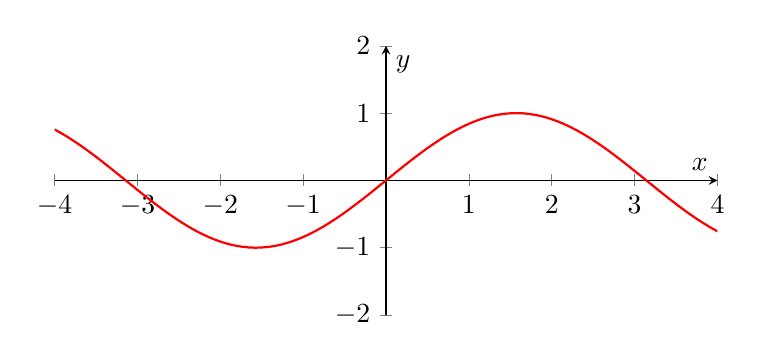
\begin{tikzpicture}
           \begin{axis}[
               axis lines = center,
               xlabel = $x$,
               ylabel = $y$,
               samples = 100,
               domain = -4:4,
               xmin = -4, xmax = 4,
               ymin = -2, ymax = 2,
               width=10cm,
               height=5cm
               ]
               \addplot[red, thick] {sin(deg(x))};
           \end{axis}
       \end{tikzpicture}
   \end{center}
   Then, $f(t) = \cos(t)$, $g(t) = \sin(t)$ are orthogonal: $2\cos(t)\sin(t) = \sin(2t)$
   \[
       \int_{-1}^{1} \cos(t)\sin(t)\:d{t} = \frac{1}{2}\int_{-1}^{1} \sin(2t) \: d{t} = 0  
   \] 
   \end{enumerate} 
\end{eg}% --- CHUNK_METADATA_START ---
% needs_review: True
% src_checksum: 34a1b6efd8afd5a191fedcc4063c7162e4ff251b3b80e839ad5d5aa5c887835f
% --- CHUNK_METADATA_END ---
\begin{definition}
    If $E$ is a Euclidean space, the set
    \[
        L(E, \R) = \{ f: E \to \R \mid f \text{ is linear}\}
    \] is called the "dual of $E$".
    It is denoted $E^*$. An element $f \in E^*$ is called a linear form.
\end{definition}% --- CHUNK_METADATA_START ---
% needs_review: True
% src_checksum: 3b0fe845bcfce365ebe09bee7ac9bde0d0486f12b24754d48e80e6331fd867ae
% --- CHUNK_METADATA_END ---
Recall:% --- CHUNK_METADATA_START ---
% needs_review: True
% src_checksum: c62046bf44d7a01ed59a1a4b7bea4075b61a00b15df8ed0bc5edfae3be41e91d
% --- CHUNK_METADATA_END ---
\begin{prop}
    If $F, F'$ are two finite-dimensional vector spaces, then $dim(L(F, F')) = dim(F)\cdot dim(F')$\\
    In particular, $dim(F^*) = dim(F)$. Indeed, if $n = (e_1, \ldots, e_p)$ is a basis of $F$ and $n' = (e'_1, \ldots, e'_q)$ is a basis of $F'$, then the mapping
    \begin{align*}
        : L(F, F') &\longrightarrow Mat_{f\times p}(\R) \\
        f &\longmapsto (f) = Mat_{n,n'}(f)
    .\end{align*}
    is an isomorphism. Therefore $dim(F, F) = qp$
\end{prop}% --- CHUNK_METADATA_START ---
% needs_review: True
% src_checksum: c9aa8b287720d3caad43357c6f50e57667cb4596ca051151224ebd08f7781253
% --- CHUNK_METADATA_END ---
\begin{theorem}
    Rank Theorem: If  $F$ is a finite-dimensional vector space and  $f: F \to F'$ is linear, then $dim(F) = dim(Ker(f)) + dim(Im(f))$
\end{theorem}% --- CHUNK_METADATA_START ---
% needs_review: True
% src_checksum: d2a5584e9f9f2893dffad3bfa59128e0eff437ca2b8cc8fdfdca03e8312c5f4a
% --- CHUNK_METADATA_END ---
\begin{prop}
    If $F, F'$ are two finite-dimensional vector spaces \underline{such that} $dim(F) = dim(F')$ and $f: F \to F'$ is linear, then $f$ is an isomorphism $\iff Ker(f) = {0}$
\end{prop}% --- CHUNK_METADATA_START ---
% needs_review: True
% src_checksum: 6c10e113159dc42fee26f775e32f5b658f01d15a5a580ec4fb86fb5c44d8a610
% --- CHUNK_METADATA_END ---
\begin{explanation}
   Recall that if $G, G'$ are finite-dimensional subspaces in the same vector space, then:
   \[
   G = G' \iff G \subseteq G' \text{ and } dim(G) = dim(G')
   \] 
   $\implies$) $f$ is injective  $\implies$ $Ker(f) = {0}$\\
   $\impliedby$) Let $Ker(f) = {0}$.\\
   Then, necessarily  $dim(Ker(f)) = 0$ and by the rank theorem, we have  $dim(F) = dim(Im(f))$, so  $Im(f) = F'$
\end{explanation}% --- CHUNK_METADATA_START ---
% needs_review: True
% src_checksum: 96310fb223d39512a621685fe14d4231b8b736cf346ef901b9446c1f0f46329a
% --- CHUNK_METADATA_END ---
\begin{lemma} Riesz's Lemma:\\
    Let $(E, \scalair{.,.})$ be a finite-dimensional Euclidean space and $f \in E^*$. Then, $\exists! u \in E$ such that $f(x) = \scalair{u, x} \quad \forall x \in E$. The linear form $f$ is given by an inner product with a vector.
\end{lemma}% --- CHUNK_METADATA_START ---
% needs_review: True
% src_checksum: db83365bab1f1a066c9d4aceecc2aaa09b915c739ca3c1af5b5b251e538fbf9e
% --- CHUNK_METADATA_END ---
\begin{notation}
   For any $v \in E$, we denote by $f_v$ the mapping:
   \begin{align*}
       f_v: E &\longrightarrow \R \\
       x &\longmapsto f_v(x) = <v, x>
   .\end{align*}
   $f_v$ is linear $\forall v \in E$, i.e. $E^*$
\end{notation}% --- CHUNK_METADATA_START ---
% needs_review: True
% src_checksum: b785e304a80823e3776a8546fe9e9abdab13358fac4e47eabd1971e31b5ed134
% --- CHUNK_METADATA_END ---
\begin{explanation} Riesz Lemma\\
   Consider the mapping
   \begin{align*}
       \phi: E &\longrightarrow E^* \\
       v &\longmapsto \phi(v) = f_v
   .\end{align*}
   $\phi$ is linear (exercise). $\phi$ is injective:
   \[
   v \in Ker(\phi) \iff f_v(x) = 0 \quad \forall x \in E
   \] 
   in particular for x = v, we have:
   \[
   0 = f_v(v) = <v,v> \implies v = 0
   \] 
   \begin{align*}
       dim(E) = dim(E^*) &\implies \phi \text{ is an isomorphism}\\
                         &\implies \phi \text{ bijective}
   \end{align*}
   \[
   \forall f \in E^*, \exists! n \in E \text{ such that } \phi(n) = f, \text{ i.e } f(x) = <n, x> \, \forall x \in E
   \] 
   In this case $E = \R^n$, the Riesz Lemma is very simple to understand:\\
   Let $f: \R^n \to \R$ be a linear form. If we denote $(e_1, \ldots, e_n)$ the canonical basis of $\R^n$, any $x \in \R^n$ can be written as
    \begin{align*}
        x = \sum_{n=1}^{n} \alpha_ie_i \qquad \alpha_i \in \R, \forall i \in \{1, \ldots, n\}\\
        \implies f(x) = \sum_{n=1}^{n} \alpha_if(e_i) = <(\alpha_1, \ldots, \alpha_n), (a_1, \ldots, a_n)> = <(a_1, \ldots, a_n), (\alpha_1, \ldots, \alpha_n)>
   \end{align*}
\end{explanation}